\documentclass[tikz]{standalone}

\usepackage{amsmath}
\usepackage{physics}

\usetikzlibrary{arrows.meta,fit,positioning}

\begin{document}
	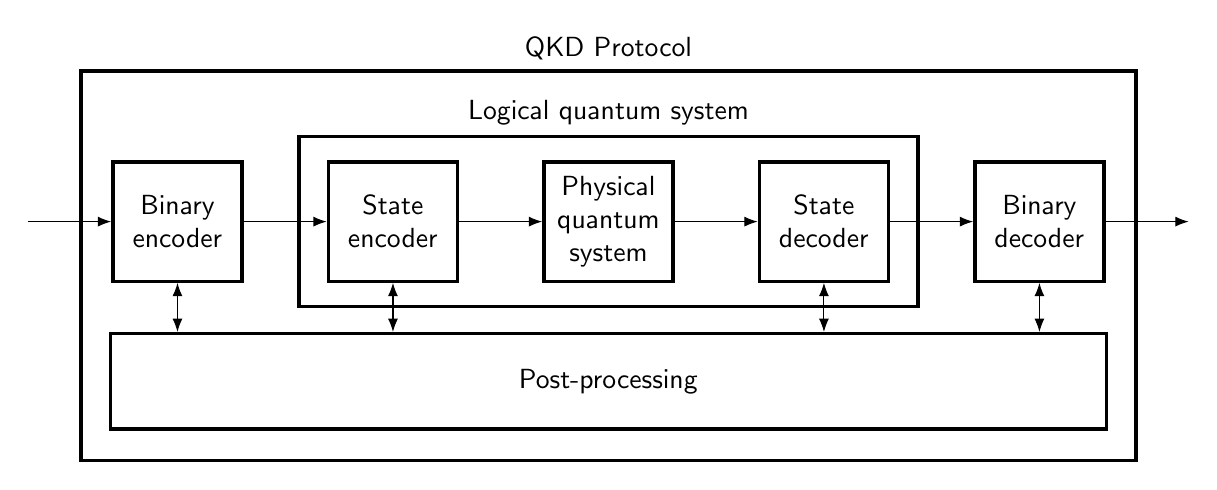
\begin{tikzpicture}[
		node distance=3em,
		block/.style={draw, very thick, minimum height=10ex, minimum width=3.5em, text width=4em, align=center},
	]
		\node[block] (phy) {\textsf{Physical quantum system}};
		\node[block, left=of phy] (senc) {\textsf{State encoder}};
		\node[block, right=of phy] (sdec) {\textsf{State decoder}};
		\node[block, fit=(senc) (sdec), inner xsep=1em, inner ysep=2ex, label={\textsf{Logical quantum system}}] (log){};
		\node[block, left=of senc] (benc) {\textsf{Binary encoder}};
		\node[block, right=of sdec] (bdec) {\textsf{Binary decoder}};
		\node[block, below=0.3 of log, minimum width=36em, text width=12em, minimum height=8ex] (pp) {\textsf{Post-processing}};
		\node[block, fit=(benc) (bdec) (pp), label={\textsf{QKD Protocol}}, inner xsep=1em, inner ysep=5ex, yshift=2.5ex] (proto) {};

		\coordinate[left=of benc] (in);
		\coordinate[right=of bdec] (out);
		
		\draw[-Latex] (in) -- (benc);
		\draw[-Latex] (benc) -- (senc);
		\draw[-Latex] (senc) -- (phy) ;
		\draw[-Latex] (phy) -- (sdec);
		\draw[-Latex] (sdec) -- (bdec);
		\draw[-Latex] (bdec) -- (out);
		\draw[Latex-Latex] (benc) -- (benc|-pp.north);
		\draw[Latex-Latex] (bdec) -- (bdec|-pp.north);
		\draw[Latex-Latex] (sdec) -- (sdec|-pp.north);
		\draw[Latex-Latex] (senc) -- (senc|-pp.north);
	\end{tikzpicture}
\end{document}
